%%\documentclass[12pt,russianb]{report}
%\usepackage[russian]{babel}
%\usepackage[cp1251]{inputenc}

\documentclass{report}
\usepackage{cmap}
\usepackage[T2A]{fontenc}

\usepackage[utf8]{inputenc}
\usepackage[english,russian]{babel}

\usepackage{longtable}   % подключение длинных таблиц
\usepackage[dvipsnames]{xcolor}
\usepackage{multirow}
\usepackage{array}
\usepackage{indentfirst} % идентификация первых абзацев после секционирования
\usepackage{lastpage}    % пакет достчета страниц 

\usepackage{fancyhdr}                    % расширенный формат страниц
\voffset=-25mm   % -25                   % сдвиг страницы вверх
\hoffset=-15mm   % -10     


  \usepackage[pdftex]{graphicx}            % загрузка графики под pdf
  \usepackage{cmap}                        % чтоб работал поиск по PDF 
  \usepackage[unicode, pdftex, colorlinks, linkcolor=blue]{hyperref}   % гиперссылки в PDF
  \pdfcompresslevel=9                      % сжимаем PDF 
  \textheight=240mm                        % для PDF высота печатного текста
  \textwidth=165mm                         % ширина печатного текста
  \renewcommand{\baselinestretch}{1.3}        % для PDF интервалы между
  \baselineskip=1.3\baselineskip              % строками 


\pagestyle{empty}
\pagestyle{fancy}
\lhead{\tiny ООО <<Опти-Софт>>}
\chead{}
\rhead{\tiny Отчет по обследованию производства \FIRMA}
\cfoot{\rule{\textwidth}{0.25pt}
~\arabic{page}}

\sloppy                             % подавление дополнительных переносов
\righthyphenmin=2                   % можно переносить
\setlength{\parindent}{10mm}        % отступ красной строки

\usepackage{todonotes}
%\newcommand{\todo}[1]{}
%\renewcommand{\todo}[1]{{\color{red} TODO: {#1}}}



\usepackage{placeins}    % пакет позволяет вставлять плавающие объекты (рисунки) в том месте, 
                         % где это необходимо. Для вывода рисунка после него встаить команду \FloatBarrier
                         
                         
                         

\newcommand{\red}[1]{\textcolor{Red}{#1}}
\newcommand{\green}[1]{\textcolor{Green}{#1}}
\newcommand{\blue}[1]{\textcolor{Blue}{#1}}                       
\newpage

\subsection{Управление взаимоотношениями с клиентами}
\label{BP_CRM}

Привлечением новых клиентов на ПРЕДПРИЯТИИ занимается отдела продаж.

Менеджеры отдела продаж ищут новых клиентов в различных открытых источниках, через обзвон потенциальных покупателей, через Интернет. 
Менеджеры для поиска новых клиентов используют холодные звонки, выставки, командировки, образцы гофропродукции с полок магазинов. Есть разработанная памятка по общению с потенциальными клиентами (рис. \ref{pic:I.2.jpg}). По факту процесс общения и взаимодействия с потенциальным клиентом менеджер выбирает сам.

Численность отдела продаж на момент обследования составляет 7 человек: 1 руководитель отдела и 6 менеджеров отдела продаж.
Направления продаж распределены между менеджерами следующим образом.

\begin{itemize}
    \item 2 человека работают на рабочих местах. Их направление продаж  ''Калужское направление'', структурно подчиняются ООО ТД ''ФОРМАТ''.
    \item 1 человек исполняет обязанности старшего менеджера. Структурно подчиняется Филиалу «Веста» ООО ''ПЗБМ''. Должностные обязанности включают в себя кроме выполнения продаж, формирование отчетности по запросам ООО ТД ''ФОРМАТ'' и Филиала «Веста» ООО ''ПЗБМ'', участие в планерных и прочих совещаниях, контроль дебиторской задолженности, контроль загруженности склада ГП и т.д.
    \item 1 человек работает удаленно. Физически располагается в городе Москва, структурно подчиняется ООО ТД ''ФОРМАТ''. Направление поиска клиентов - ''Московское направление''.
    \item 2 человека  работают удаленно. Физически располагаются в городе Брянск. Структурно подчиняются ООО ТД ''ФОРМАТ''. Направление поиска клиентов - ''Центральный регион'' и трейдеры, что составляет 10-20 \% от общего объема выпускаемой ПРЕДПРИЯТИЕМ продукции.
    
\end{itemize}


Не смотря на то, что существует распределение по направлениям продаж, соблюдается оно условно.


Системы CRM на предприятии не выявлено. Общей базы новых (потенциальных) клиентов на предприятии не ведется. Аналитики направления развития продаж нет. Каждый менеджер ведет свою базу в удобной для себя форме (рис. \ref{pic:I.3..jpg}). Учет взаимоотношений с клиентами ведется на ручном уровне и в удобной для каждого менеджера форме. Информация по новым клиентам у менеджеров находится только в электронных письмах и личных записях. Опросный лист для клиента не используется, собирается только информация, достаточная, для анализа возможности изготовления на предприятия и быстрого расчета стоимости.   

Почта приходит на общий электронный адрес. 
Звонки и электронная почта поступают лично каждому менеджеру.
Количество новых клиентов примерно 5-6 в месяц.



 

%CRM системы не выявлено.


%Единой базы потенциальных покупателей не выявлено.

%Новых клиентов менеджер заводит в справочник Контрагенты в системе СБИС только при заключении договора.

% Новые клиенты заносятся как лиды. МАП заносит карточку покупателя в модуле CRM системы 1С: УНФ. МАП ведет историю взаимоотношений с клиентами вручную записывая историю звонков, рассылок.
% В CRM созданы шаблоны сценариев работы с покупателем. Каждое событие работы с контрагентом является  элементом справочника с тем  шаблоном.
% При появлении потенциального клиента МАП определяет лицо принимающее решение со стороны организации. МАП запрашивает требования по изготовлению изделия и получает техническое задание (размеры и характеристики нового изделия). 

 %В отделе продаж есть четкий регламент работы по новым заказчикам.
% Одна сделка представляет собой несколько изделий готовой продукции для одного клиента.

%
%
%
%
%%
%Менеджеры отдела маркетинга 
%занимаются поиском и привлечением новых покупателей. Выделяется пассивный поиск через сайт, рекламу и участие в мероприятиях, и активный поиск через адресную рассылку.
%Все контакты хранятся на сетевом ресурсе в сети ПРЕДПРИЯТИЯ, куда есть доступ большинству пользователей сети.
%При появлении нового покупателя менеджеры отдела маркетинга создают каталог в сетевом каталоге клиентов.
%Внутри каталога хранится информация по письмам с клиентами, договорам, спецификациям и тендерам.
%
%%
%Новых заказчиков ведет менеджер отдела продаж и закупок.
%После выполнения предварительных заказов заказчику ведущий специалист отдела продаж передает клиентов менеджерам отдела продаж.
%%
%%\begin{figure}
%%\begin{center}
%%\ifnum\pdfoutput=0
%%  \includegraphics[40,0][366,292]{Pics/TK1.png}
%%\else 
%%  \includegraphics[height=0.94\textheight, keepaspectratio]{Pics/CustomerList.jpg}
%%\fi
%%\end{center}
%%  \caption{Разделение потребителей гофротары в разрезе маркетологов}
%%  \label{pic:CustomerList}
%%\end{figure}
%%\clearpage
%%
%%
\begin{figure}
\begin{center}
 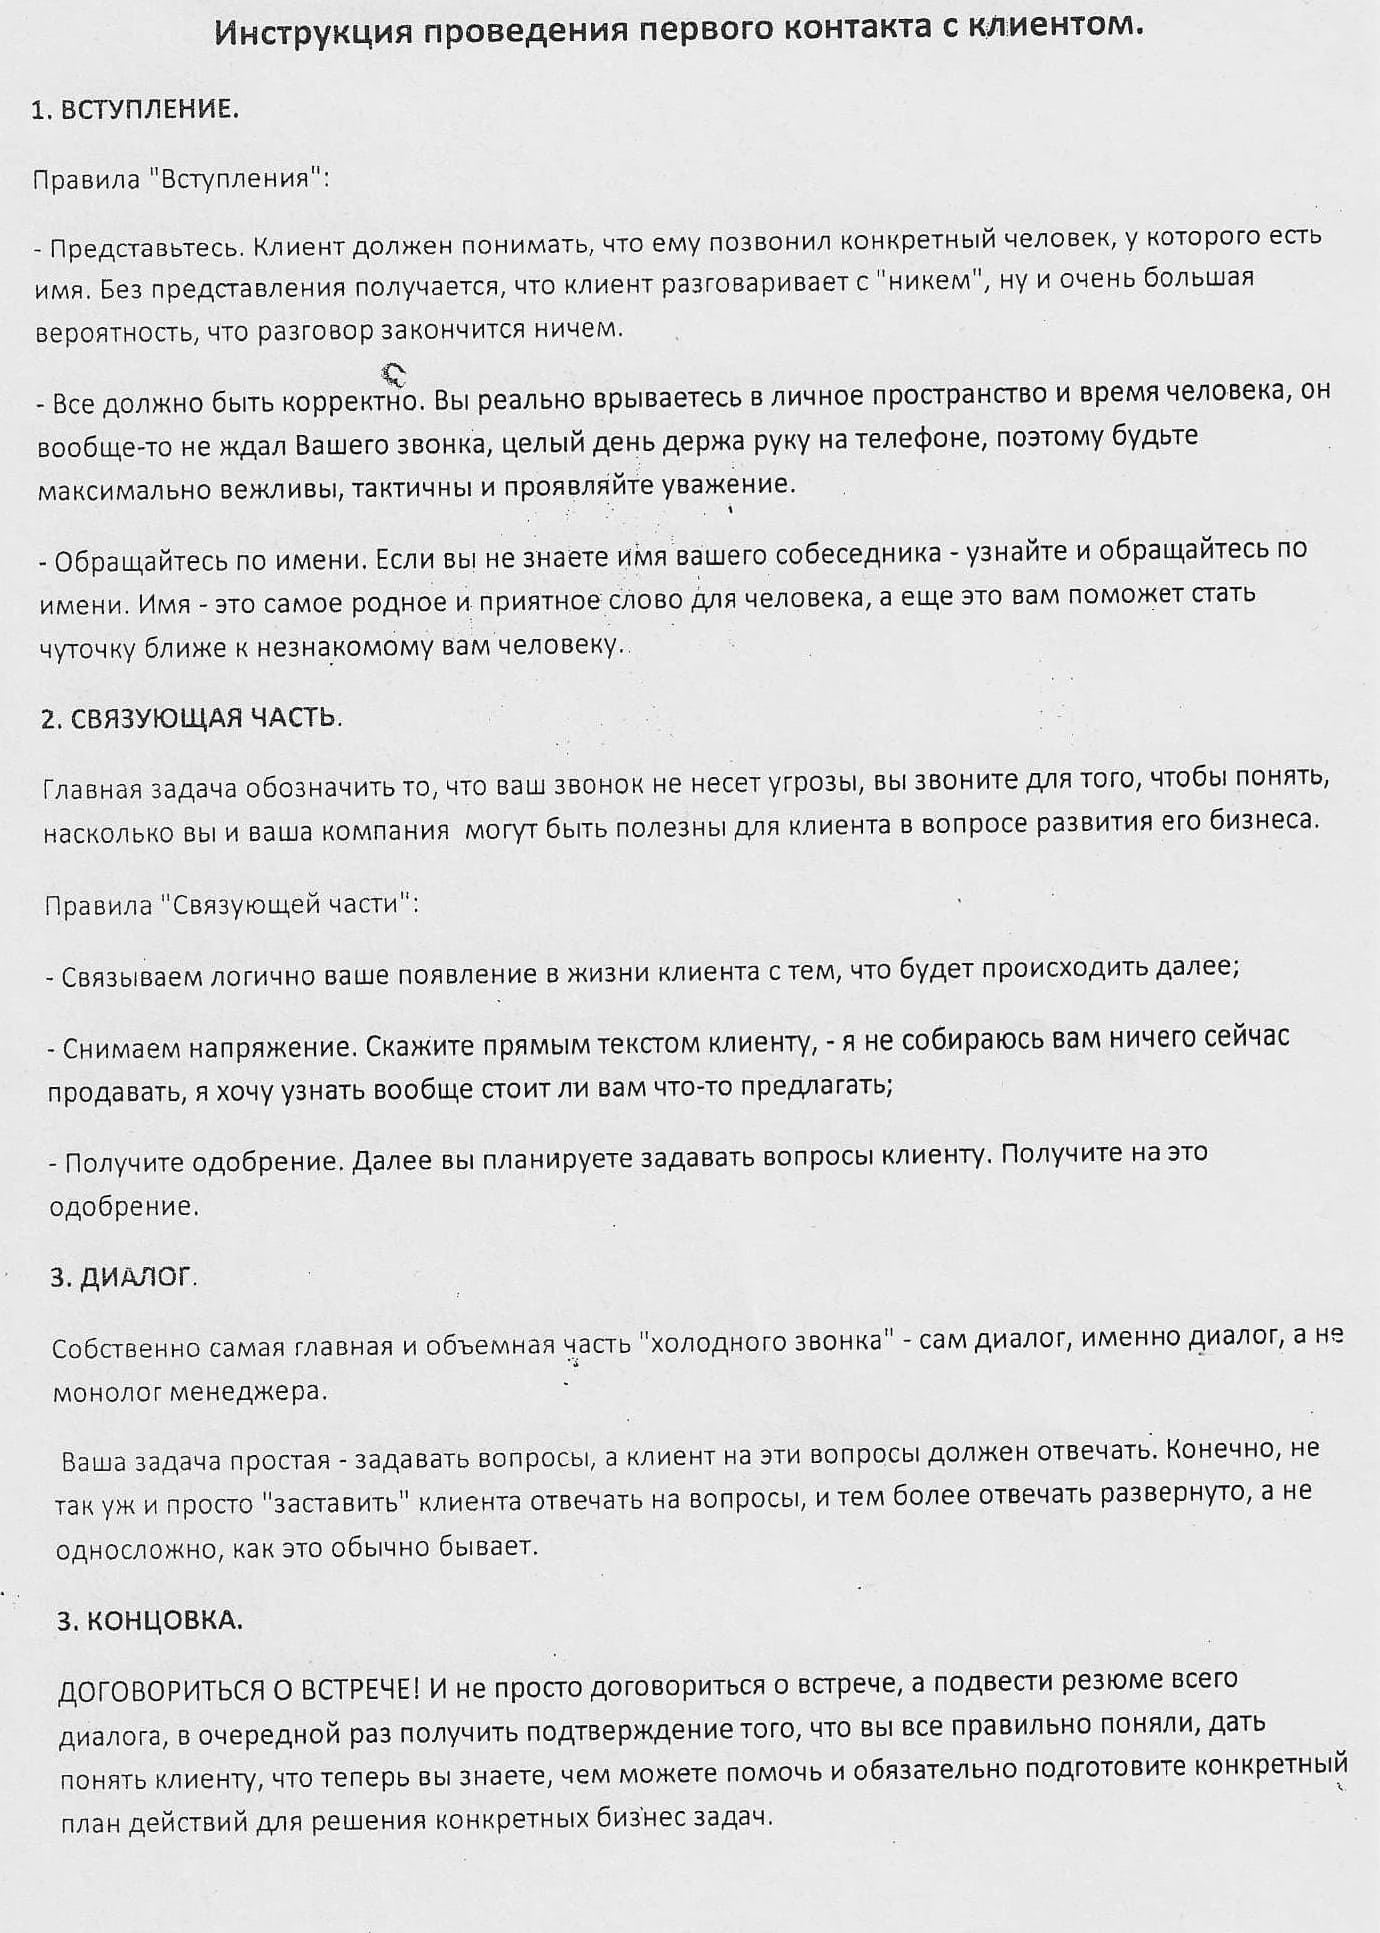
\includegraphics[height=0.8\textheight, keepaspectratio]{Pics/I.2.jpg}
\end{center}
 \caption{Памятка менеджеру}
 \label{pic:I.2.jpg}
\end{figure}
\clearpage

\begin{figure}[!h]
\begin{center}
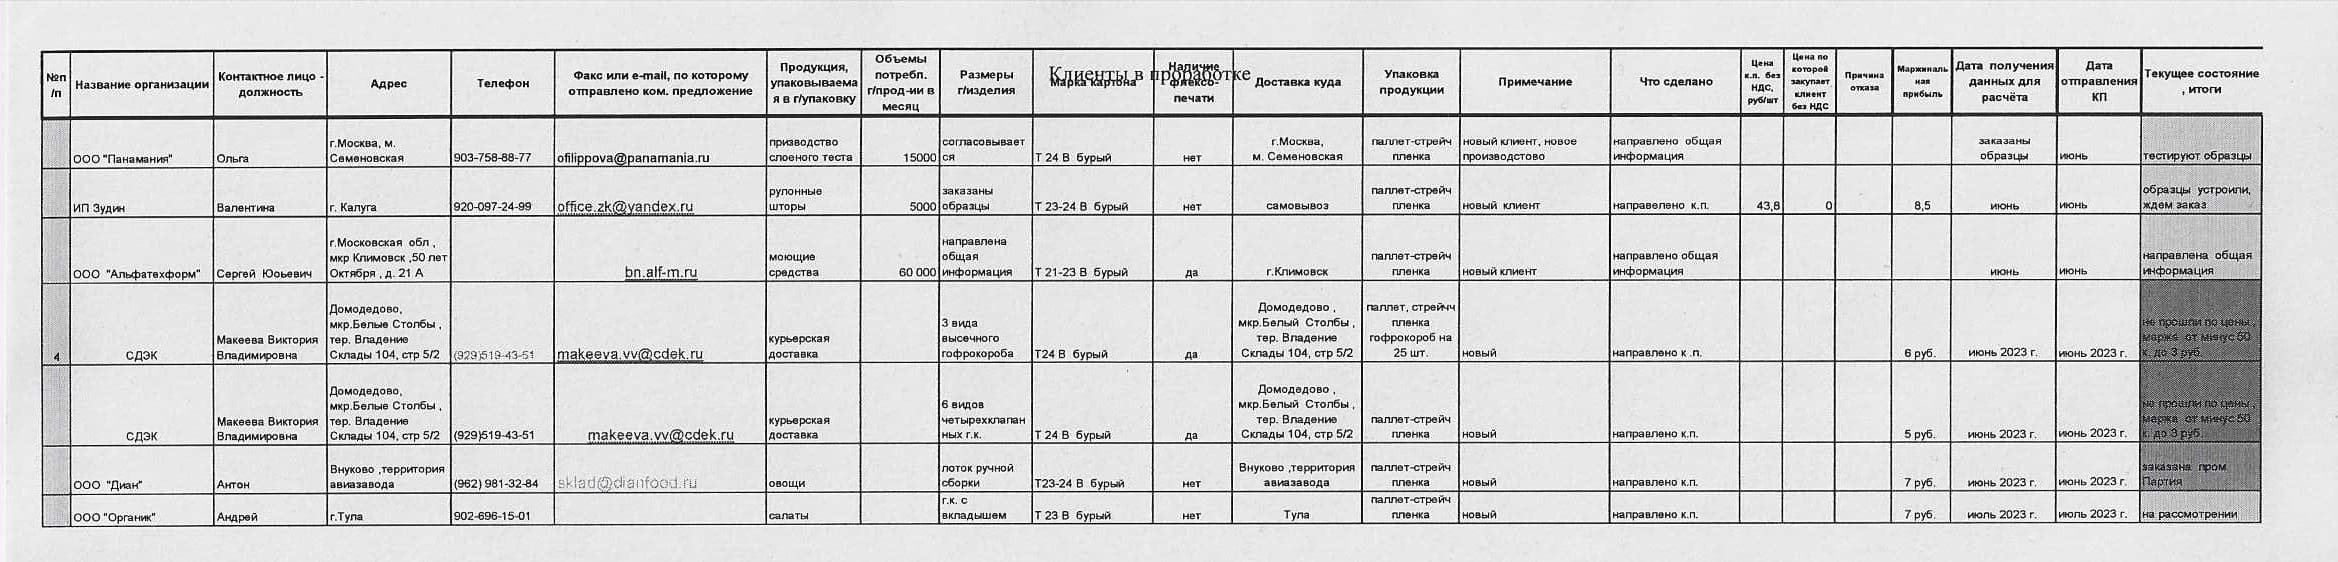
\includegraphics[height=0.3\textheight, width=1.1\textwidth, angle=90, keepaspectratio]{Pics/I.3..jpg}
\end{center}
 \caption{Пример реестра новых (потенциальных) клиентов }
 \label{pic:I.3..jpg}
\end{figure}
\clearpage

%
%
%
%


%\clearpage
\ifx \notincludehead\undefined
\normalsize
\end{document}
\fi 